% overall design, architectural design, interface design, database design
% implementation - frontend (main, canvas, checklist) and backend (template creation, template storing, 3, 4)
% user diagram

% \section{Limitations}

\section{Design}
% justify out of context wborkflow process

\subsection{Software's Structure}
\begin{figure}[ht]
    \centering
    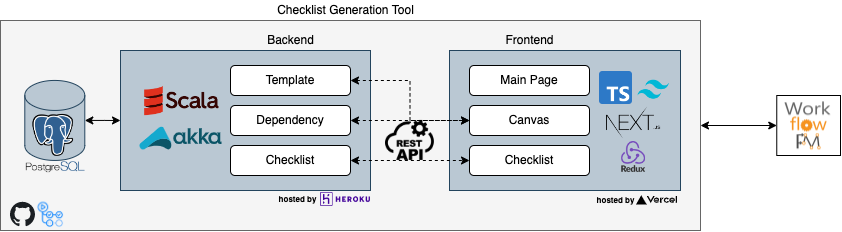
\includegraphics[width=\textwidth]{overleaf/images/softwares_structure.png}
    \caption{Software's Structure}
    \label{fig:software_structure}
\end{figure}

\subsection{Architectural Design}
- choices: React, Vue, Angular, Scala.js

- chose: React, Next.js, TailwindCSS, Redux

- choices: Node.js, Scala, Java

- choices for Scala: akka-http, http4s, play

chose: Scala, Akka-http

- GitHub, GitHub Actions, PostgreSQL, ElephantSQL, Vercel, Heroku

\subsection{Interface Design}

- Chen's design \cite{checklistdesign}

- Form creators; e.g. google forms, microsoft forms

- differences between the original design and the final design

\subsection{Database Design}
- main checklist design

- templates, components

- input\_information\_parent, input\_information\_child, input\_information\_child\_query

\begin{figure}[ht]
    \centering
    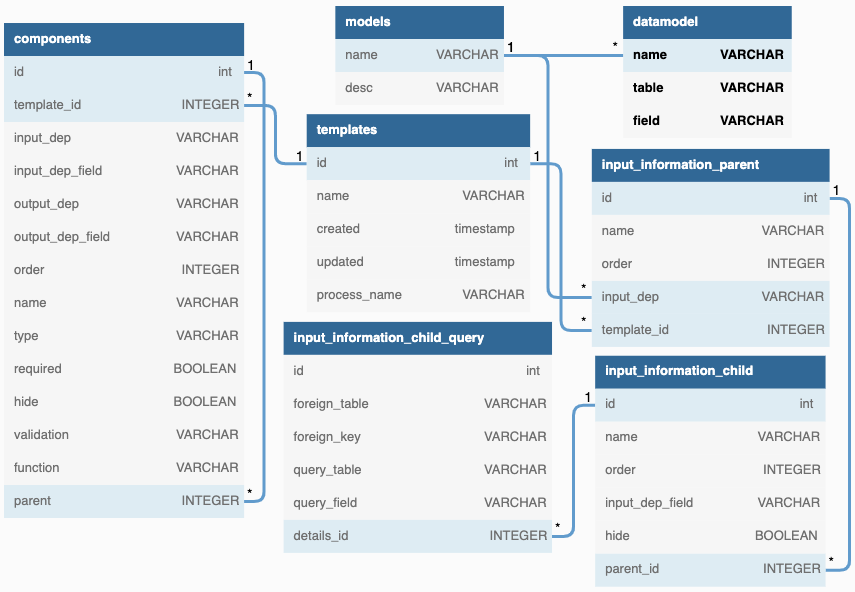
\includegraphics[width=\textwidth]{overleaf/images/checklist_db_design.png}
    \caption{Checklist Database Design}
    \label{fig:checklist_db_design}
\end{figure}

\section{Functional Specification}


\section{Implementation}
\subsection{Frontend}

\subsubsection{Main Screen}

\subsubsection{Canvas Screen}

\subsubsection{Preview Screen}

\subsubsection{Checklist Screen}

\subsection{Backend}

\subsubsection{Application Programming Interfaces}
- workflow process to checklist template

- get dependencies

- get foreign tables/keys

- saving template

- retrieve finished templates


\subsection{Naive Suggestion}
\subsubsection{Naive Queryable Field Suggestion}
\subsubsection{Naive Dependency Suggestion}

\section{Diagrams}
\subsection{Use Case Diagram}
\begin{figure}[ht!]
    \centering
    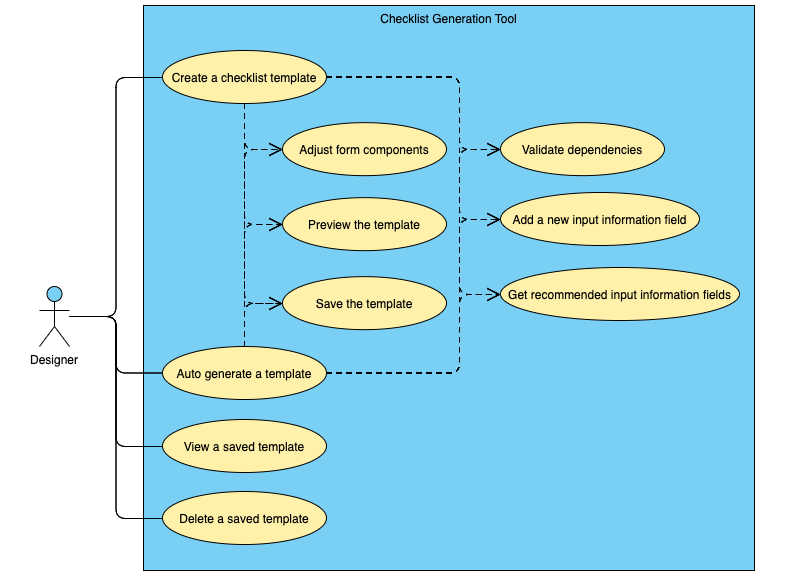
\includegraphics[width=\textwidth]{overleaf/images/use_case_diagram.png}
    \caption{Use Case Diagram}
    \label{fig:use_case_diagram}
\end{figure}

\subsection{Sequence Diagrams}
\begin{figure}[ht!]
    \centering
    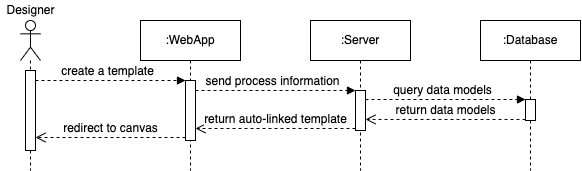
\includegraphics[width=\textwidth]{overleaf/images/create_template.png}
    \caption{Sequence Diagram of Create Template Scenario}
    \label{fig:create_template}
\end{figure}

\noindent
\textbf{Scenario \#1:} Figure \ref{fig:create_template} \\
\textbf{Goal:} \\
\textbf{Preconditions:} \\
\textbf{Breakdown:} \\

\begin{figure}[ht!]
    \centering
    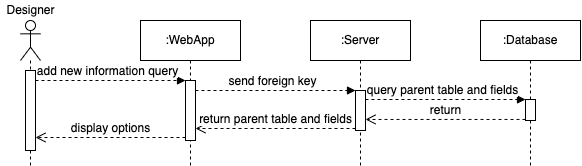
\includegraphics[width=\textwidth]{overleaf/images/add_new_information_query.png}
    \caption{Sequence Diagram of Add New Information Query Scenario}
    \label{fig:add_new_information_query}
\end{figure}

\noindent
\textbf{Scenario \#2:} Figure \ref{fig:add_new_information_query} \\
\textbf{Goal:} \\
\textbf{Preconditions:} \\
\textbf{Breakdown:} \\

\begin{figure}[ht!]
    \centering
    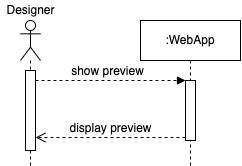
\includegraphics[width=0.4\textwidth]{overleaf/images/show_preview.png}
    \caption{Sequence Diagram of Show Preview Scenario}
    \label{fig:show_preview}
\end{figure}

\noindent
\textbf{Scenario \#3:} Figure \ref{fig:show_preview} \\
\textbf{Goal:} \\
\textbf{Preconditions:} \\
\textbf{Breakdown:} \\

\begin{figure}[ht!]
    \centering
    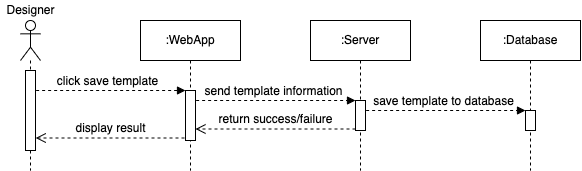
\includegraphics[width=\textwidth]{overleaf/images/save_template.png}
    \caption{Sequence Diagram of Save Template Scenario}
    \label{fig:save_template}
\end{figure}

\noindent
\textbf{Scenario \#4:} Figure \ref{fig:save_template} \\
\textbf{Goal:} \\
\textbf{Preconditions:} \\
\textbf{Breakdown:} \\

\begin{figure}[ht!]
    \centering
    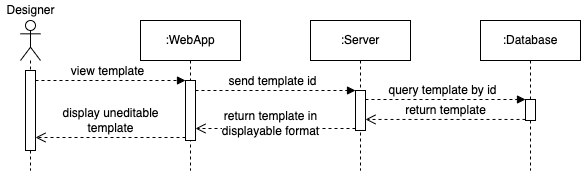
\includegraphics[width=\textwidth]{overleaf/images/view_template.png}
    \caption{Sequence Diagram of View Template Scenario}
    \label{fig:view_template}
\end{figure}

\noindent
\textbf{Scenario \#5:} Figure \ref{fig:view_template} \\
\textbf{Goal:} \\
\textbf{Preconditions:} \\
\textbf{Breakdown:} \\

\section{Challenges}

tree structure of workflowfm's processes, doing all suggestions within sql queries, design challenges (queryable input fields), http4s sucks-akka-http works
